\documentclass{article}

\usepackage[letterpaper, portrait, margin=1in]{geometry}
\usepackage{siunitx}
\usepackage{tikz}
\usepackage{mathtools}
\usetikzlibrary{shapes,backgrounds}
\usepackage{amsmath}
\begin{document}

\title{Dyanmics Equations for Smartmouse 2018}
\author{Peter Mitrano}

\maketitle

Deriving the kinematic equations of a differential drive robot.

\hfill
-
\begin{figure}[h]
  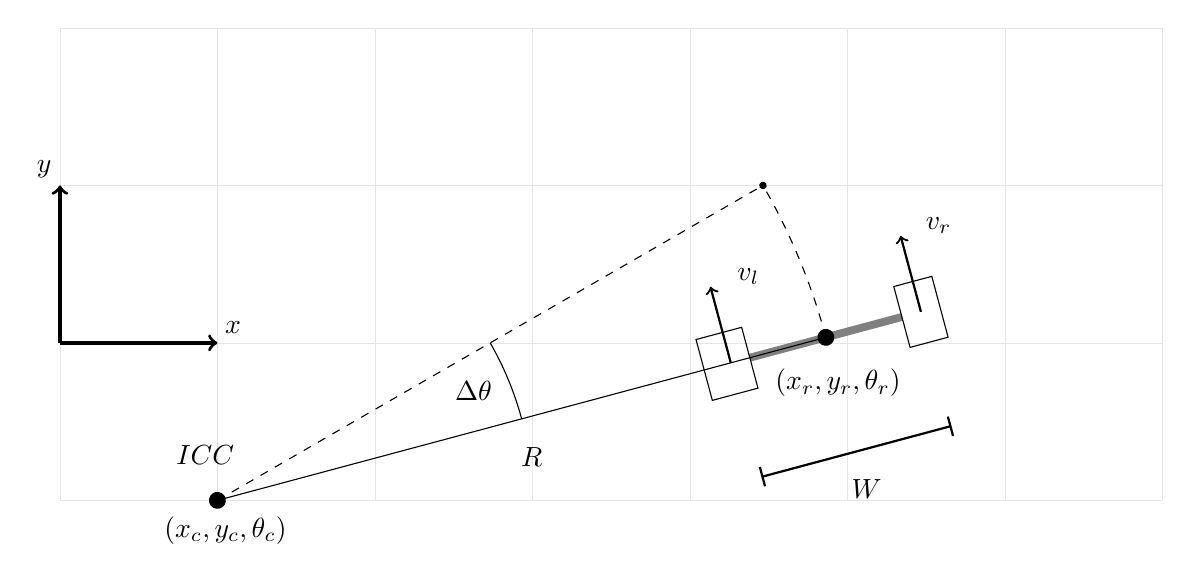
\begin{tikzpicture} [scale=2]
    % coordinate frame and grid%
    \definecolor{lg}{rgb}{0.9,0.9,0.9}
    \draw[step=1,lg,very thin] (-1,0) grid (6,3);
    \draw [very thick,->] (-1,1) -- (-1,2);
    \draw [very thick,->] (-1,1) -- (0,1);
    \draw (-1.1, 2.1) node {$y$};
    \draw (0.1, 1.1) node {$x$};

    % robot and stuff %
    \draw [line width=1mm, draw=gray,rotate around={15:(0,0)}]{(3.5,0)--(4.5, 0)};
    \draw [rotate around={15:(0,0)}] {(3.2,-0.2) rectangle (3.5, 0.2)};
    \draw [rotate around={15:(0,0)}] {(4.5,-0.2) rectangle (4.75, 0.2)};
    \draw [rotate around={15:(0,0)}] {(0,0) -- (4, 0)};
    \draw [dashed,rotate around={30:(0,0)}] {(0,0) -- (4, 0)};
    \draw [dashed,rotate around={15:(0,0)}] (4,0) arc (0:15:4);
    \draw [rotate around={15:(0,0)}] (2,0) arc (0:15:2);
    \draw [thick,->,rotate around={15:(0,0)}] (3.375,0) -- (3.375,0.5);
    \draw [thick,->,rotate around={15:(0,0)}] (4.625,0) -- (4.625,0.5);
    \draw [thick,|-|,rotate around={15:(0,0)}] (3.375,-0.75) -- (4.625,-0.75);
    \filldraw [rotate around={15:(0,0)}] {(0,0) circle (.05)};
    \filldraw [rotate around={15:(0,0)}] {(4,0) circle (.05)};
    \filldraw [rotate around={30:(0,0)}]{(4,0) circle (.02)};
    \draw [rotate around={15:(0,0)}] (1.75, 0.25) node {$\Delta\theta$};
    \draw [rotate around={15:(0,0)}] (3.625, 0.5) node {$v_l$};
    \draw [rotate around={15:(0,0)}] (4.875, 0.5) node {$v_r$};
    \draw [rotate around={15:(0,0)}] (2, -0.25) node {$R$};
    \draw [rotate around={15:(0,0)}] (4, -1) node {$W$};
    \draw [rotate around={15:(0,0)}] (4, -.3) node {$(x_r,y_r,\theta_r)$};
    \draw [rotate around={15:(0,0)}] (0, 0.3) node {$ICC$};
    \draw [rotate around={15:(0,0)}] (0, -.2) node {$(x_c,y_c,\theta_c)$};
  \end{tikzpicture}
  \centering
\end{figure}

At an instant in time we say that the robot is turning around some point $ICC$, the instanteous center. The radius $R$ about that point is what we want to solve for. We start with the knowedge that since the robot doesn't tear itself apart while driving, the rate $\omega$ at which both wheels (and the robot) move around $ICC$ is the same.
\begin{equation} \label{eq:1}
  \omega_l = \omega_r = \omega
\end{equation}
Let $R_l$ and $R_l$ be the radius to the right and left wheels.
\begin{equation} \label{eq:2}
  \omega_l = \frac{v_l}{R_l}, \omega_r = \frac{v_r}{R_r}
\end{equation}
We can then combine \ref{eq:1} and \ref{eq:2}
\begin{equation}
  \frac{v_l}{R_l} = \frac{v_r}{R_r}
\end{equation}
We can then substitute $R_l = R - \frac{W}{2}$ and $R_r = R + \frac{W}{2}$
\begin{equation}
  \frac{v_l}{R-\frac{W}{2}} = \frac{v_r}{R + \frac{W}{2}}
\end{equation}

Now do some algebra...
\begin{align*}
  \frac{v_l}{R-\frac{W}{2}} &= \frac{v_r}{R + \frac{W}{2}} \\[1em]
  \frac{R-\frac{W}{2}}{v_l} &= \frac{R + \frac{W}{2}}{v_r} \\[1em]
  \frac{R}{v_l}-\frac{W}{2v_l} &= \frac{R}{v_r} + \frac{W}{2v_r} \\[1em]
  \frac{R}{v_l}-\frac{R}{v_r} &= \frac{W}{2v_r}+\frac{W}{2v_l} \\[1em]
  \frac{2R(v_r-v_l)}{v_rv_l} &= \frac{W(v_l+v_r)}{2v_rv_l} \\[1em]
  R(v_r-v_l) &= W(v_l+v_r) \\[1em]
  R &= \frac{W(v_l+v_r)}{2(v_r-v_l)} \\[1em]
\end{align*}

\textbf{Next we need to figure out how to update our $x_r$, $y_r$, and $\theta_r$ given $R$.} \\

Before we can solve any of these, we need to figure out what $\Delta\theta$ is equal to. We will assume we are following this arc of constant radius for a given time step $\Delta t$. This is a good assumption if our time step is equal to our controller time step, during which presumably the speeds of the motors aren't changing, and so neither will our turning radius. If so, then $\Delta\theta = \omega\Delta t$, and we know
$$\omega=\dfrac{v_l}{R-\frac{W}{2}} = \dfrac{v_r}{R+\frac{W}{2}}$$
Lets just pick $v_l$, and put them together to get $\Delta\theta$.
$$\Delta\theta = \dfrac{v_l}{R-\frac{W}{2}}\Delta t$$

Theta is obvious: $\theta_r \leftarrow \theta_r+\Delta\theta$. The coordinates of $ICC = (x_r-R\sin{\theta_r}, y_r+R\cos{\theta_r})$. You can see this if you think that the vector to $ICC$ is 90 degrees offset from $\theta_r$ and do the trig. Let's assume in the situation diagramed above, $\theta_r=\ang{105}$, $R=4$, and $x=4.8, y=0$, so $ICC = (4.8-4\sin{(105)}, 0+4\cos{(105)}) \approx (1, -1)$. For another example, pretend the robot is right below the origin facing east at $(0,-1,0)$ and $R=1$. $ICC$ should be $(0,0)$ so let's check. $ICC = (0-1\sin{(0)}, -1+1\cos{(0)}) = (0, 0).$ Great, the math seems to check out. Now we just rotate the robot coordinates around the point $ICC$ by $\Delta\theta$, which we can do easily with a rotation matrix. Of course, we're not rotating around the origin, we're roating around $ICC$, so we first subtract out the coordinates of $ICC$ to get $(x_o, y_o) = (x_r- ICC_x, y_r-ICC_y)$. Recall that to rotate around the origin by $\Delta\theta$, we multiply our point $(x_o, y_o)$ as follows:
\begin{equation}
  \begin{bmatrix}
    \cos{\Delta\theta} & \sin{\Delta\theta} \\
    -\sin{\Delta\theta} & \cos{\Delta\theta} \\
  \end{bmatrix}
  \begin{bmatrix}
    x_o \\
    y_o \\
  \end{bmatrix}
  =
  \begin{bmatrix}
    x_{new} \\
    y_{new} \\
  \end{bmatrix}
\end{equation}
We then just add back the coordinates of $ICC$. Great! Now we know how to update all our coordinates. Let's summarize:

\begin{align}
 \theta_r &\leftarrow \theta_r + \Delta\theta \\
  x_r &\leftarrow \cos{(\Delta\theta)}(x_r-ICC_x)+\sin{(\Delta\theta)}(y_r-ICC_y) + ICC_x \\
  y_r &\leftarrow -\sin{(\Delta\theta)}(x_r-ICC_x)+\cos{(\Delta\theta)}(y_r-ICC_y) + ICC_y \\
\shortintertext{where}
  ICC_x &= x_r-R\sin{\theta_r} \\
  ICC_y &= y_r+R\cos{\theta_r} \\
  \Delta\theta &= \dfrac{v_l}{R-\frac{W}{2}}\Delta t \\
  R &= \frac{W(v_l+v_r)}{2(v_r-v_l)}
\end{align}

We can expand and simplify the udpate equations for $x_r$.

\begin{align}
  x_r &\leftarrow \cos{(\dfrac{v_l}{R-\frac{W}{2}}\Delta t)}(x_r-x_r+R\sin{\theta_r})+\sin{(\dfrac{v_l}{R-\frac{W}{2}}\Delta t)}(y_r-y_r-R\cos{\theta_r}) + x_r-R\sin{\theta_r} \\
  x_r &\leftarrow \cos{(\dfrac{v_l}{R-\frac{W}{2}}\Delta t)}(R\sin{\theta_r})+\sin{(\dfrac{v_l}{R-\frac{W}{2}}\Delta t)}(-R\cos{\theta_r}) + x_r-R\sin{\theta_r} \\
  x_r &\leftarrow R\cos{(\dfrac{v_l}{R-\frac{W}{2}}\Delta t)}\sin{\theta_r}-R\sin{(\dfrac{v_l}{R-\frac{W}{2}}\Delta t)}\cos{\theta_r} + x_r-R\sin{\theta_r} \\
  x_r &\leftarrow x_r+R\cos{(\dfrac{v_l}{R-\frac{W}{2}}\Delta t)}\sin{\theta_r}-R\sin{(\dfrac{v_l}{R-\frac{W}{2}}\Delta t)}\cos{\theta_r}-R\sin{\theta_r} \\
  x_r &\leftarrow x_r+R\Big(\cos{(\dfrac{v_l}{R-\frac{W}{2}}\Delta t)}\sin{\theta_r}-\sin{(\dfrac{v_l}{R-\frac{W}{2}}\Delta t)}\cos{\theta_r}\Big)-R\sin{\theta_r} \\
  \shortintertext{let $\dfrac{v_l}{R-\frac{W}{2}}=a$, and $\theta_r=b$, we can use $\cos{a}\sin{b}-\sin{a}\cos{b}=-\sin{(a-b)}$}
  x_r &\leftarrow x_r+R\Bigg(-\sin{\Big(\dfrac{v_l}{R-\frac{W}{2}}\Delta t-\theta_r}\Big)\Bigg)-R\sin{\theta_r} \\
  x_r &\leftarrow x_r+R\Bigg(-\sin{\Big(\dfrac{v_l}{R-\frac{W}{2}}\Delta t-\theta_r}\Big)-\sin{\theta_r}\Bigg) \\
  x_r &\leftarrow x_r-R\Bigg(\sin{\Big(\dfrac{v_l}{R-\frac{W}{2}}\Delta t-\theta_r}\Big)+\sin{\theta_r}\Bigg) \\
  \shortintertext{sub in for $R$ in the denominator}
  x_r &\leftarrow x_r-R\Bigg(\sin{\Big(\dfrac{v_l}{\frac{W(v_l+v_r)}{2(v_r-v_l)}-\frac{W}{2}}\Delta t-\theta_r}\Big)+\sin{\theta_r}\Bigg) \\
  x_r &\leftarrow x_r-R\Bigg(\sin{\Big(\dfrac{v_l}{\frac{W(v_l+v_r)}{2(v_r-v_l)}-\frac{W(v_r-v_l)}{2(v_r-v_l)}}\Delta t-\theta_r\Big)}+\sin{\theta_r}\Bigg) \\
  x_r &\leftarrow x_r-R\Bigg(\sin{\Big(\dfrac{v_l}{\frac{Wv_l+Wv_r-Wv_r+Wv_l)}{2(v_r-v_l)}}\Delta t-\theta_r\Big)}+\sin{\theta_r}\Bigg) \\
  x_r &\leftarrow x_r-R\Bigg(\sin{\Big(\dfrac{v_l}{\frac{Wv_l}{(v_r-v_l)}}\Delta t-\theta_r\Big)}+\sin{\theta_r}\Bigg) \\
  x_r &\leftarrow x_r-R\Bigg(\sin{\Big(\frac{v_r-v_l}{W}\Delta t-\theta_r\Big)}+\sin{\theta_r}\Bigg)
\end{align}

We can apply the same process for $y_r$.

\begin{align}
  x_l &\leftarrow x_l-R\Bigg(\cos{\Big(\frac{v_r-v_l}{W}\Delta t-\theta_r\Big)}-\cos{\theta_r}\Bigg)
\end{align}

\textbf{Final Solution to the forward Kinematics:}
\begin{align}
 \theta_r &\leftarrow \theta_r + \dfrac{v_l}{R-\frac{W}{2}}\Delta t \\
  x_r &\leftarrow x_r-R\Bigg(\sin{\Big(\frac{v_r-v_l}{W}\Delta t-\theta_r\Big)}+\sin{\theta_r}\Bigg) \\
  x_l &\leftarrow x_l-R\Bigg(\cos{\Big(\frac{v_r-v_l}{W}\Delta t-\theta_r\Big)}-\cos{\theta_r}\Bigg)
\end{align}


\end{document}

